\subsection{Casi d'uso}
Di seguito vengono riportati i casi d'uso raggruppati in base all'attore. Gli attori in gioco sono i seguenti:
\begin{itemize}
	\item volontario;
	\item caposquadra;
	\item coordinatore.
\end{itemize}

\subsubsection{Casi d'uso: Volontario}
\begin{itemize}
	\item \textbf{UC1 - Gestione account}:
	come volontario, voglio poter visualizzare e modificare le informazioni relative al mio account.
	
	\item \textbf{UC2 - Login}:
	come volontario, voglio poter accedere al mio profilo personale.
	
	\item \textbf{UC3 - Logout}:
	come volontario, voglio poter disconnettere il mio profilo personale dall'applicazione.
	
	\item \textbf{UC4 - Gestione reperibilità}:
	come volontario, voglio poter indicare e modificare le mie ore di reperibilità.
	
	\item \textbf{UC5 - Visualizzazione informazioni squadra}:
	come volontario, voglio poter visualizzare le informazioni relative alla mia squadra.
	
	\item \textbf{UC6 - Visualizza intervento programmato}:
	come volontario, voglio poter visualizzare le informazioni relative ad un intervento programmato a cui sono stato assegnato.
	
	\item \textbf{UC7 - Visualizza emergenza}:
	come volontario, voglio poter visualizzare le informazioni relative ad un intervento d'emergenza a cui sono stato assegnato.
	
	\item \textbf{UC8 - Visualizza informazioni zona}:
	come volontario, voglio poter consultare le informazioni riguardanti il meteo, terremoti, qualità dell'aria, stazioni personalizzate relative alla zona assegnata alla mia squadra.
	
	\item \textbf{UC9 - Inserimento informazioni report}:
	come volontario, voglio poter arricchire la documentazione relativa ad un intervento, aggiungendo osservazioni e foto.
	
	\item \textbf{UC10 - Segnalazione operatività}:
	come volontario, voglio poter segnalare quando sono operativo e mi trovo sul luogo dell'intervento.
\end{itemize}




\subsubsection{Casi d'uso: Caposquadra}
Il caposquadra include tutti i casi d'uso del volontario più i seguenti:
\begin{itemize}
	\item \textbf{UC11 - Gestione report intervento programmato}:
	come caposquadra, voglio poter visualizzare e modificare i report riguardanti gli interventi programmati creati da me.
	
	\item \textbf{UC12 - Gestione report emergenza}:
	come caposquadra, voglio poter visualizzare e modificare i report riguardanti le emergenze create da me.
	
	\item \textbf{UC13 - Gestione intervento programmato}:
	come caposquadra, voglio poter creare, modificare o eliminare un intervento programmato.
	
	\item \textbf{UC14 - Gestione intervento emergenza}:
	come caposquadra, voglio poter creare, modificare o eliminare un intervento d'emergenza.
	
	\item \textbf{UC15 - Visualizzazione posizione real-time}:
	come caposquadra, voglio poter visualizzare su una mappa la posizione in tempo reale dei volontari operativi appartenenti alla mia squadra durante un intervento.
	
	\item \textbf{UC16 - Amministrazione squadra}:
	come caposquadra, voglio poter visualizzare e modificare le giacenze del magazzino e compilare il bilancio relativo alla mia squadra.
	
	\item \textbf{UC17 - Notifiche allarmi zona}:
	come caposquadra, voglio poter decidere su quali eventuali allarmi, relativi alla mia zona, essere notificato.
	
	\item \textbf{UC18 - Gestione informazioni relative alla zona}:
	come caposquadra, voglio poter definire quali informazioni (meteorologiche, terremoti, stazioni personalizzate, bollettini protezione civile) ricevere.
\end{itemize}




\subsubsection{Casi d'uso: Coordinatore}
\begin{itemize}
	\item \textbf{UC1 - Gestione account}:
	c coordinatore, voglio poter visualizzare e modificare le informazioni relative al mio account.
	
	\item \textbf{UC2 - Login}:
	come coordinatore, voglio poter accedere al mio profilo personale.
	
	\item \textbf{UC3 - Logout}:
	come coordinatore, voglio poter disconnettere il mio profilo personale dall'applicazione.
	
	\item \textbf{UC19 - Inserimento volontari}:
	come coordinatore, voglio poter inserire nuovi volontari.
	
	\item \textbf{UC20 - Gestione squadre}:
	come coordinatore, voglio poter creare, modificare ed eliminare le squadre.
\end{itemize}


\clearpage
\subsection{Diagramma dei casi d'uso}
In figura \ref{fig:UseCaseDiagram} è stato riportato il diagramma dei casi d'uso. In questo diagramma sono stati inseriti i casi d'uso descritti in precedenza mettendoli in correlazione con il corrispettivo attore. È importante notare che la figura del \textit{caposquadra} è una specializzazione del \textit{volontario} e di conseguenza eredita tutti i suoi casi d'uso, oltre ad implementarne altri personalizzati. 

\begin{sidewaysfigure}[h!]
	\centering
	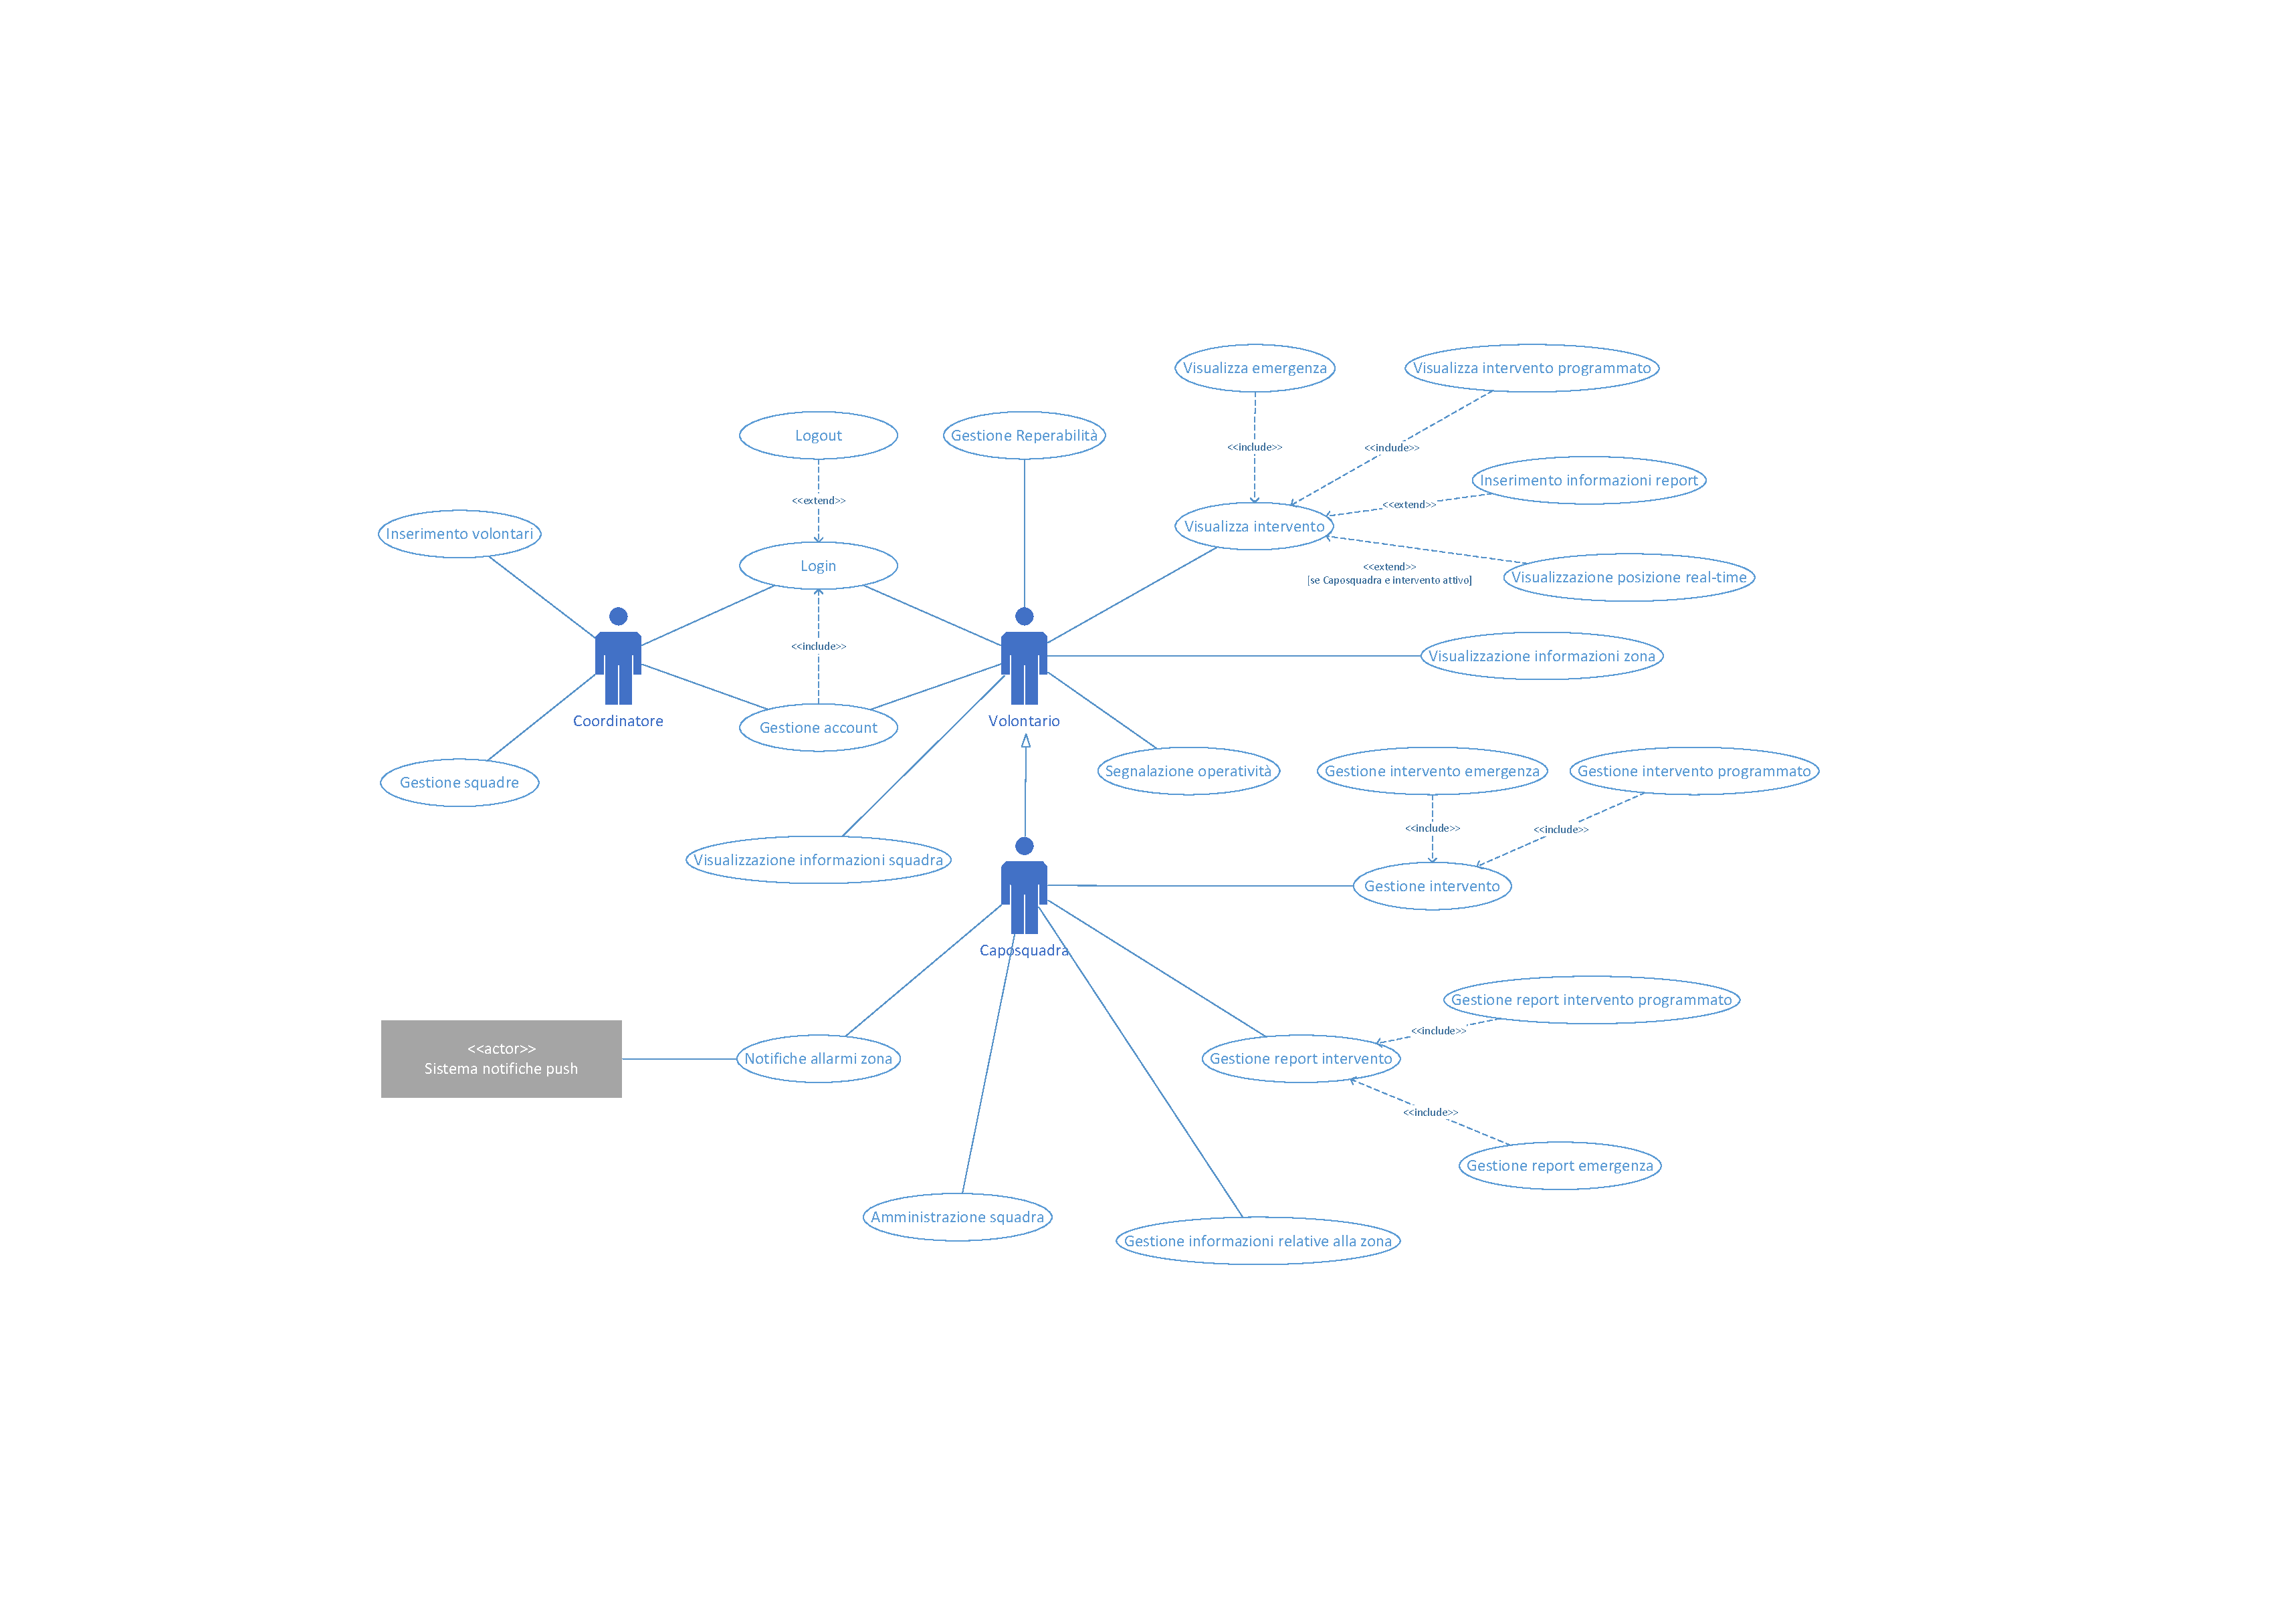
\includegraphics[width=0.9\linewidth]{OtherFiles/Use cases diagram}
	\caption{Diagramma dei casi d'uso.}
	\label{fig:UseCaseDiagram}
\end{sidewaysfigure}


